\documentclass[tikz,border=10pt]{standalone}
\begin{document}
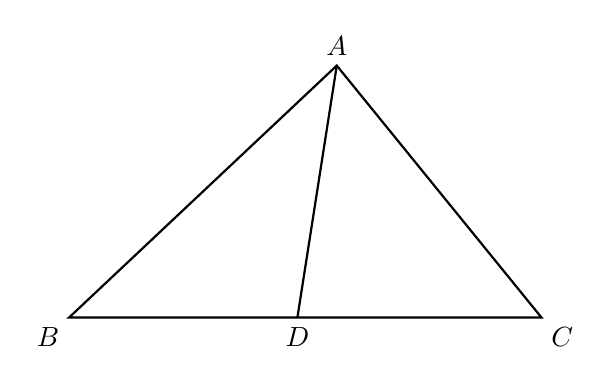
\begin{tikzpicture}
  \coordinate (B) at (0,0);
  \coordinate (C) at (6,0);
  \coordinate (A) at (3.4,3.2);
  \coordinate (D) at (2.9,0);

  \draw[thick] (A) -- (B) -- (C) -- cycle;
  \draw[thick] (A) -- (D);

  \node[below left] at (B) {$B$};
  \node[below right] at (C) {$C$};
  \node[above] at (A) {$A$};
  \node[below] at (D) {$D$};
\end{tikzpicture}
\end{document}
